\documentclass[a4paper,11pt]{article}
\usepackage[utf8]{inputenc}
\usepackage[T1]{fontenc}
\usepackage[frenchb]{babel}

\usepackage{graphicx}
\usepackage{fancyhdr}
\usepackage{geometry}

\usepackage[colorlinks,linkcolor=blue]{hyperref}
\usepackage{amsmath}
\usepackage{amssymb}
\usepackage{mathrsfs}
%\usepackage{epsfig}
%\usepackage {eurosym}

\usepackage{float}

\geometry{a4paper,tmargin=2cm,bmargin=2cm,lmargin=1.5cm,rmargin=1cm,headheight=2.2cm,headsep=0.5cm,footskip=1cm}
\columnsep=0.6cm

\graphicspath{{images/}} 

\usepackage{listings}
\usepackage{color}
\usepackage{xcolor}

\lstset{columns=flexible,keepspaces=true, breaklines,breakindent=0pt} 


\lstset{language=VHDL,
basicstyle=\ttfamily\footnotesize,
breaklines, 
keywordstyle=\bfseries\color{blue},
stringstyle=\color{red},
commentstyle=\color{blue!20!black!30!green},
morecomment=[s][\color{black}]{/**}{*/},
numbers=left,
numberstyle=\tiny\color{black},
stepnumber=2,
numbersep=10pt,
tabsize=4,
showspaces=false,
showstringspaces=false}


\fancypagestyle{plain}{
% noms des respo   dans le bas de page                                            
\lfoot{Projet de VHDL}
\rfoot{M.Morin J.Fourmann}
\renewcommand{\headrulewidth}{0pt}
\fancyhead{}}
% Titre a compl»ter
\title{\textbf{ \huge{Projet de VHDL}}  \\{\Large Réalisation d'un Fréquencemètre}}

\author{
\textsc{Jérémie Fourmann} (Promo 2013 - Eléctronique)\\ %mettre votre nom
\textsc{Maxime Morin} (Promo 2013 - Eléctronique)\\ %mettre votre nom
%\textsc{ddd dddd} (Promo - departement - respo)     %2 nom
}

\graphicspath{{images/}}

\begin{document}

\pagestyle{plain}

\maketitle
\begin{center}

\includegraphics[width=6cm]{inp-enseeiht.pdf}   
\end{center}

\vspace{1cm}
\renewcommand{\contentsname}{Plan}
\tableofcontents
\vspace{2cm}

\newpage
\section{Objectifs}
Le but de ce projet est de réaliser un dispositif capable de mesurer avec précision la fréquence d'un signal.
Il sera réalisé sur un FPGA de type Spartan-3e implanté sur une carte de développement Nexys2.
Nous disposons donc d'une interface comportant des entrées sorties utilisateur comme des boutons poussoirs et des 
afficheurs 7 segments.

\subsection{Rappel du cahier des charges}

\paragraph{} Notre projet doit répondre aux contraintes suivantes :

\begin{description}
\item[Plage de fréquence : ] de 1 Hz à 10 MHz
\item[Rafraichissement de la mesure :] Toutes les secondes, pour un fonctionnement fluide pour l'utilisateur.
\item[Affichage : ] Sur 4 digits avec affichage du calibre de mesure parmis trois possibles : Hz, kHz, MHz.
\end{description}

\paragraph{}Bien qu'en apparence très simple, ce cahier des charges implique d'autres fonctions :
\begin{description}
\item[Précision : ] Il faudra que l'erreur soit de l'ordre de $10^{-3}$ pour n'affichier que des chiffres significatifs
à l'utilisateur.
\item[Méthodes de mesure : ] Pour garantir une erreur minimale sur toute la plage de fréquence, il faudra avoir recours
à deux méthodes différentes. Il faudra aussi que le dispositif soit capable de choisir la méthode la plus adaptée. 
\item[Détection des erreurs : ] Le fréquencemètre devra aussi détecter lorsqu'il sort de sa plage de 
fonctionnement normal pour le pas afficher des données érronées à l'utilisateur.
\end{description}


\subsection{Nos choix}
\subsubsection{Méthodes de mesures}
  \paragraph{} Nous avons deux méthodes de mesures à notre disposition : méthode étalon et méthode échantillonnage.

  \begin{figure}[H]
  \begin{center}
	  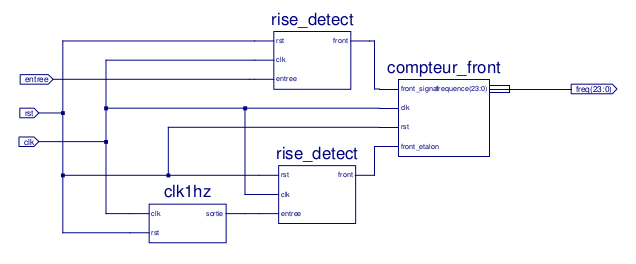
\includegraphics[scale=.4]{etalon.png}
	  \caption{Mesure de fréquence par étalonnage}
  \end{center}
  \end{figure}

  \begin{figure}[H]
  \begin{center}
	  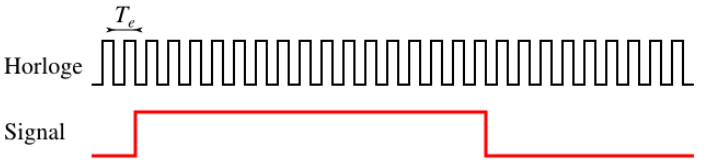
\includegraphics[scale=.4]{ech.png}
	  \caption{Mesure de fréquence par échantillonnage}
  \end{center}
  \end{figure}

  \paragraph{} Ces deux méthodes ne sont pas meilleures l'une par rapport à l'autre : elles sont complémentaires.
  En effet pour un signal de fréquence élevée nous utiliserons la méthode étalon, elle permet d'avoir le maximum de précision.
  En revanche à basse fréquence cette méthode ne peut s'apliquer convenablement, nous utiliserons alors la méthode échantillonnage.

  \paragraph{}Il faut donc trouver la valeur pour laquelle on change de méthode de mesure. Nous allons tracer la précision en fonction de la fréquence pour 
  les deux méthodes. Nous pouvons évaluer la résolution de chaqune de ces deux méthodes par les équations suivantes :

  \begin{equation*}
  Precision_{BF}= \frac{F_{clk}}{F_{signal}}
  \end{equation*}
  \begin{equation*}
  Precision_{HF}= \frac{F_{signal}}{F_{étalon}}
  \end{equation*}

\begin{figure}[H]
\begin{center}
	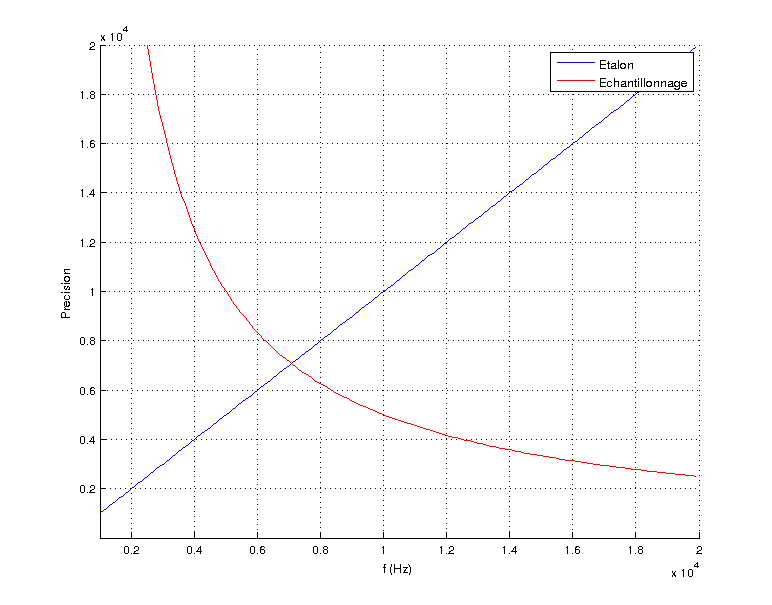
\includegraphics[scale=.7]{graphMethode.png}
	\caption{Précision des deux méthodes}
\end{center}
\end{figure}

\paragraph{}On s'apperçoit que pour avoir le maximun de précision il faut changer de méthode aux alentours de 7 KHz. 

\subsubsection{Choix de la conception en machine d'état}
Notre conception étant entièrement synchrone, chaque sous module séquentiel de notre sytème sera une machine d'état avec le 
bloc M et G synchronisé sur la clock du FPGA.
Cette conception en machine d'état nous assure des résultats après implémentation au plus proche des simulations.
Par ailleurs nous avons aussi une meilleur lisibilité de notre programme et la méthodologie de débuggage est simplifiée 
car nous avons accès à l'état de notre machine lors des simulations.


\newpage


\section{Conception du système}

\subsection{Présentation du système}

  \paragraph{}Le système final que nous implémenteons sur le FPGA ressemble à ceci :

\begin{figure}[H]
\begin{center}
	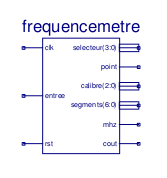
\includegraphics[scale=1]{sch-freqa0.png}
	\caption{Diagramme A-0}
\end{center}
\end{figure}

\paragraph{} L'utilisateur n'aura qu'à envoyer le signal dont il veut mesurer la fréquence. Pour une approche plus technique, décomposons
ce bloc en sous modules :

\begin{figure}[H]
\begin{center}
	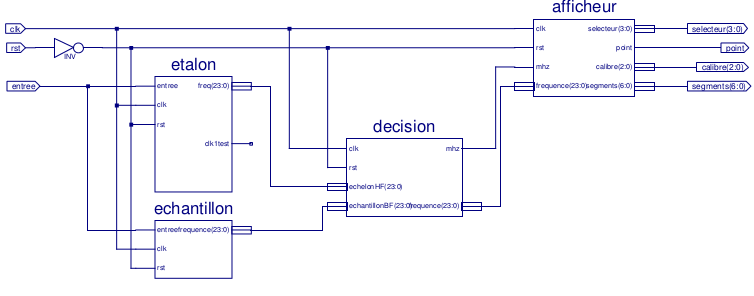
\includegraphics[scale=.9]{sch-frequencemetre.png}
	\caption{Diagramme A0}
\end{center}
\end{figure}

\paragraph{} Notre fréquencemètre se décompose en 4 blocs principaux que nous développerons par la suite : 
\begin{description}
  \item[La mesure par étalon : ] Nous mesurons le nombre de fronts du signal pendant une période étalon de 1 seconde. Ce nombre de fronts est
  proportionnel à la fréquence.
  \item[La mesure par échantillonnage : ] Nous comptons le nombre de fronts d'horloge entre dexus fronts du signal. Ce nombre est
  inversement proportionnel à la fréquence, il faudra l'inverser...
  \item[La décision : ] Nous choisissons quelle mesure est la plus précise pour être afficher, selon la fréquence de travail...
  \item[L'affichage : ] Nous affichons la valeur envoyée par le module de décision.
\end{description}

\paragraph{} Par la suite, nous allons détailler ces modules dans le même ordre que nous les avons conçus.

\subsection{Module d'affichage}
  \subsubsection{Schéma bloc}
  
  \begin{figure}[H]
\begin{center}
	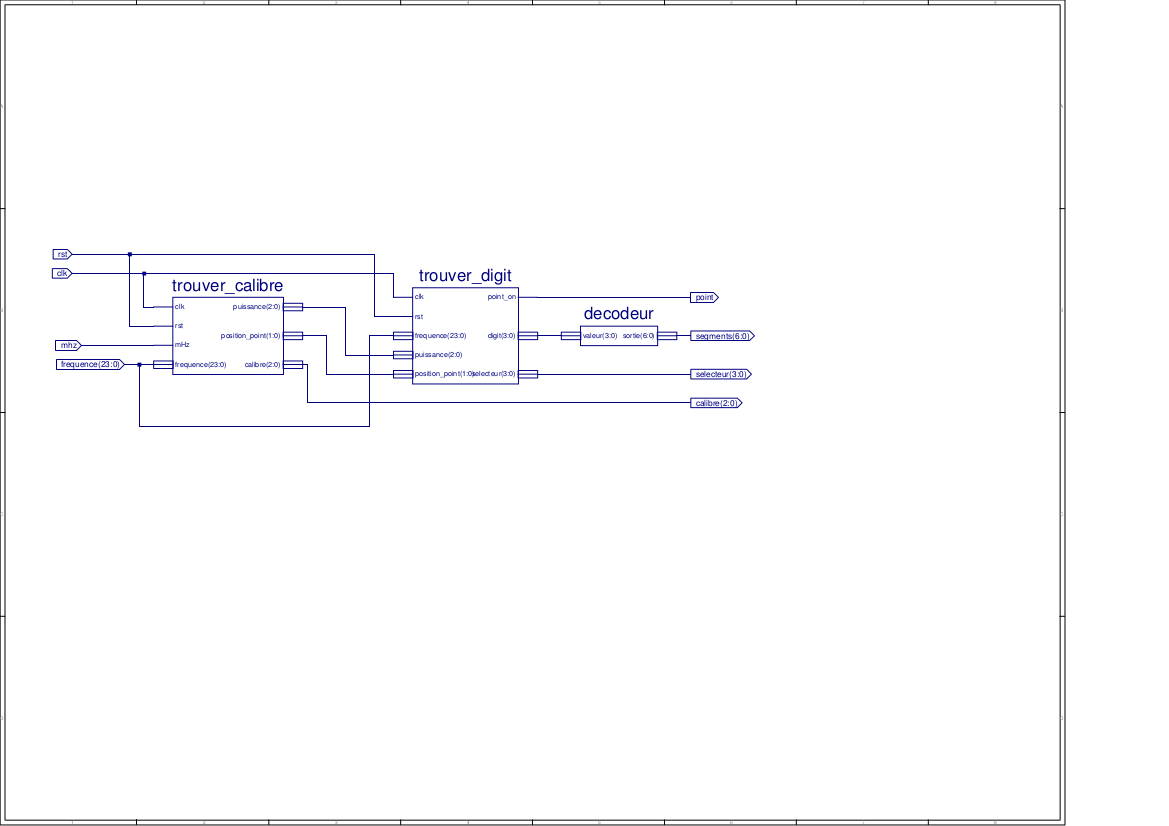
\includegraphics[scale=.9]{sch-afficheur.png}
	\caption{Diagramme A1 : module d'affichage}
\end{center}
\end{figure}

\paragraph{} L'objectif de ce module est de transformer le résultat de la mesure (une succession de zéros et de uns sans unité) 
en une grandeur physique en décimale dans les grandeurs du système internationnal... Nous avons choisi de faire un bloc très générique : 
il recevra un nombre binaire codé sur 24 bits et une information sur son unité (Hertz ou milli-Hertz), il devra ensuite le formater 
et l'afficher sur les 4 afficheurs de la carte, en plaçant le point et déterminant le calibre.

\begin{description}
  \item[trouver\_calibre : ] Ce bloc détermine le calibre que nous allons afficher à l'utilisateur, c'est à dire la position du point, la
  led à allumer, et la puissance de 10 du nombre à afficher (utile pour la conversion dans le bloc suivant). Ce bloc est combinatoire.
  \item[trouver\_digit : ] Ce module converti en binaire codé décimal et affiche un à un les quatres digits significatifs de la fréquence. 
  Il utilise des données déteminées par le bloc précédent. Il gère aussi le balayage en insérant un reatrd de 2ms entre deux digits et 
  en commandant le sélecteur.
  \item[decodeur : ] Ce bloc se contente de convertir le BCD pour commander l'afficheur. Il est combinatoire.
\end{description}


  \subsubsection{Machine d'état}
\paragraph{} Ci dessous, le graphe d'état de la seule machine d'état du module d'affichage.
\begin{figure}[H]
\begin{center}
	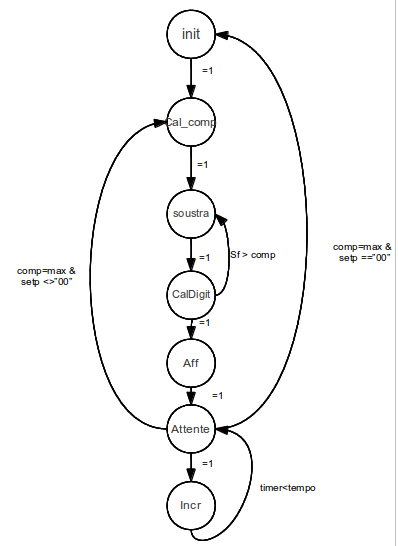
\includegraphics[scale=.8]{machine_CalDigit.png}
	\caption{Machine d'état de calcul\_digit}
\end{center}
\end{figure}

\paragraph{} Le signal \textit{step} permet de sélectionner le digit de l'afficheur qui restera éclairé pendant 2ms. Cette 
machine d'état est d'après nous la plus intéressante de ce projet. Son code source est donné en annexe.

\subsection{Mesure par étalon}
  \subsubsection{Schéma bloc}
  
  \begin{figure}[H]
\begin{center}
	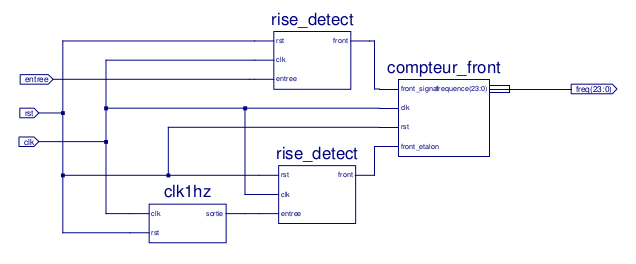
\includegraphics[scale=1]{sch-etalon.png}
	\caption{Diagramme A2 : mesure par étalon}
\end{center}
\end{figure}

\paragraph{} L'objectif de ce module est de compter le nombre de front du signal pendant un temps fixe apellé ``étalon''.
La période de cet étalon a été fixé précédemment (TODO) à une seconde. Etant donné que cette méthode ne sera utilisée que pour les 
fréquences suppérieures au KHz (le seuil étant à 7kHz), nous ferons en sorte que la grandeur de sortie soit en Hz, ce qui nous permet 
de rentrer dans le chaier des chagres en tremes de précison et en terme de plage de fréquence en n'utilisant que 24bits. Ce module 
ferta appel aux sous modules suivants :

\begin{description}
  \item[rise\_detect : ] Ce bloc permet de générer une impulsion durant exactement 1 cycle d'horloge lorsqu'un front montant est détecté
  sur son entrée.
  \item[clk1hz : ] Module de division de fréquence permettant de générer une fréquence de 1 Hertz pour cadencer les échelons.
  \item[compteur\_fronts : ] Ce bloc compte le nombre de fronts du signal entre deux fronts du signal d'étalon, après chaque mesure,
  il met la valeur sur le bus de sortie et relance une nouvelle mesure.
\end{description}


  \subsubsection{Machines d'états}

\begin{figure}[H]
   \begin{minipage}[b]{0.40\linewidth}
      \centering 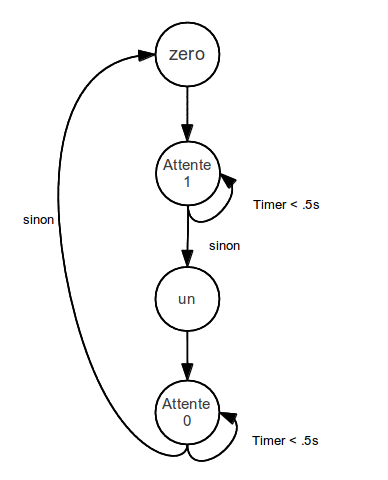
\includegraphics[scale=.6]{machine_1Hz.png}
      \caption{Machine d'état de Clock 1kHz}
   \end{minipage}\hfill
   \begin{minipage}[b]{0.40\linewidth}   
      \centering 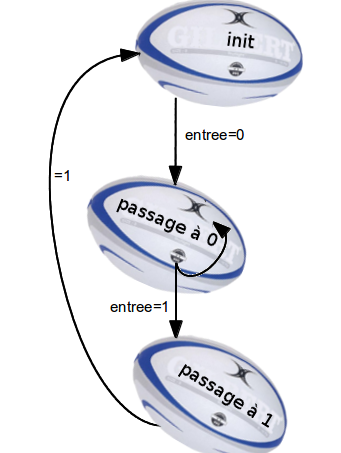
\includegraphics[scale=.6]{machine_front.png}
      \caption{Machine d'état de Rise\_detect}
   \end{minipage}
 \end{figure}

\begin{figure}[H]
\begin{center}
	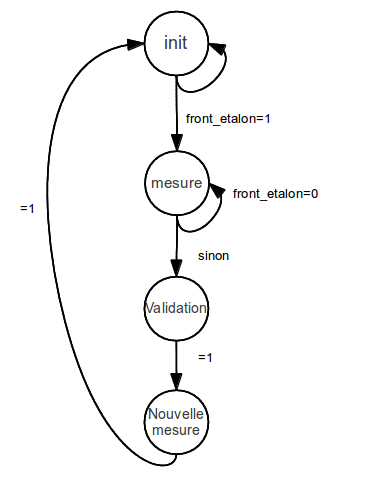
\includegraphics[scale=.6]{machine_mesureEtalon.png}
	\caption{Machine d'état de Compte\_etalon}
\end{center}
\end{figure}


  \subsection{Mesure par échantillonnage}
  \subsubsection{Schéma bloc}
  
  \begin{figure}[H]
\begin{center}
	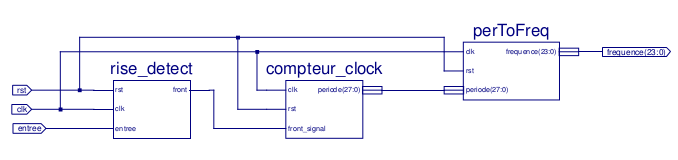
\includegraphics[scale=1]{sch-echantillon.png}
	\caption{Diagramme A3 : mesure par echantillonnage}
\end{center}
\end{figure}

\paragraph{} L'objectif de ce module est de compter le nombre de front du signal pendant un temps fixe apellé ``étalon''.
La période de cet étalon a été fixé précédemment (TODO) à une seconde. Etant donné que cette méthode ne sera utilisée que pour les 
fréquences suppérieures au KHz (le seuil étant à 7kHz), nous ferons en sorte que la grandeur de sortie soit en Hz, ce qui nous permet 
de rentrer dans le chaier des chagres en tremes de précison et en terme de plage de fréquence en n'utilisant que 24bits. Ce module 
ferta appel aux sous modules suivants :

\begin{description}
  \item[rise\_detect : ] Ce bloc permet de générer une impulsion durant exactement 1 cycle d'horloge lorsqu'un front montant est détecté
  sur son entrée.
  \item[clk1hz : ] Module de division de fréquence permettant de générer une fréquence de 1 Hertz pour cadencer les échelons.
  \item[compteur\_fronts : ] Ce bloc compte le nombre de fronts du signal entre deux fronts du signal d'étalon, après chaque mesure,
  il met la valeur sur le bus de sortie et relance une nouvelle mesure.
\end{description}


  \subsubsection{Machines d'états}
  
  \begin{figure}[H]
   \begin{minipage}[b]{0.5\linewidth}
      \centering 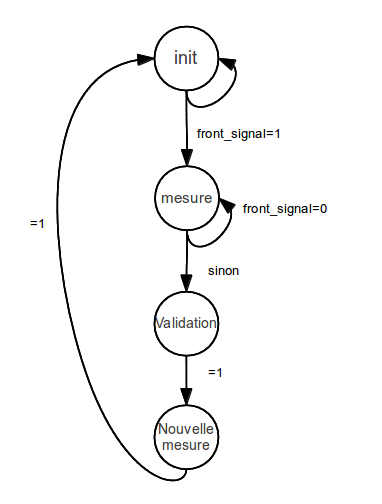
\includegraphics[scale=.6]{machine_compteurClk.png}
      \caption{Machine d'état de compteur\_clock}
   \end{minipage}\hfill
   \begin{minipage}[b]{0.5\linewidth}   
      \centering 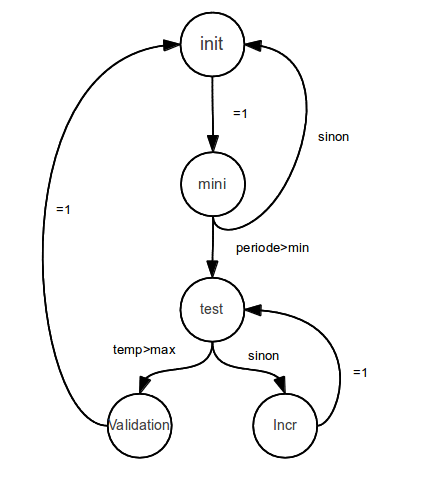
\includegraphics[scale=.6]{machine_PertoFreq.png}
      \caption{Machine d'état de PerToFreq}
   \end{minipage}
 \end{figure}

<<<<<<< HEAD

  \subsection{Décision}
 \paragraph{} Nous rapellons la composition final du fréquencemètre :
 
 \begin{figure}[H]
\begin{center}
	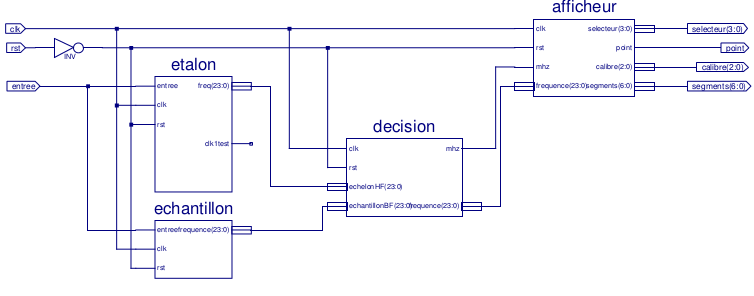
\includegraphics[scale=1]{sch-frequencemetre.png}
	\caption{Diagramme A0}
\end{center}
\end{figure}

  \paragraph{}Le seul bloc manquant est celui de décision permettant de choisir quelle méthode va être 
  sélectionner pour l'affichage. Voici la machine d'état de ce bloc :
  
   \begin{figure}[H]
\begin{center}
	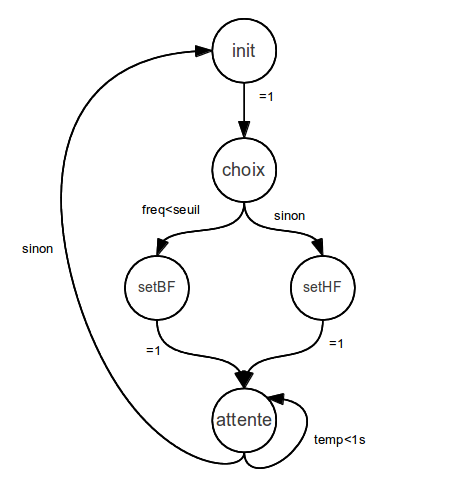
\includegraphics[scale=.6]{machine_decision.png}
	\caption{Machine d'état du bloc de décison}
\end{center}
\end{figure}
  
  
\subsection{Performances du système}
TODO : courbe erreur + pourcentage + rapidite 


=======
\subsection{Performances du système}
Nous avons une suite de mesures à différentes fréquences pour regarder l'erreur commise. Une fois calibrage effectuer, on a une erreur maximale
de 0.15\%, ce qui nous convient parfaitement.  
\begin{figure}[H]
\begin{center}
	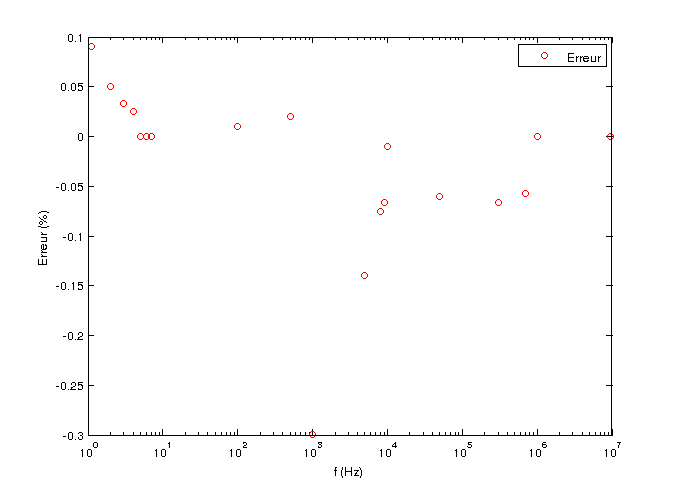
\includegraphics[scale=.7]{mesure_erreur.png}
	\caption{Erreur de mesure de nôtre fréquencemètre}
\end{center}
\end{figure}
On s'aperçoit que l'on a un pic d'erreur aux alentours de 7KHz, fréquence à laquelle on bascule de méthode pour augmenter la précision.
>>>>>>> 79805d13f5c761feaadb7bbd8c1158ea6f25fe16
\newpage
\section{Bilan}

\newpage
\appendix
\section{Manuel d'utilisateur}
\subsection{Introduction}
L'utilisateur pourra utiliser le projet soit en utilisant le component Fréquencemètre pour l'inclure dans un autre projet soit l'utilisé directement sur la Nexys 2.

\subsection{Component VHDL}
Notre projet peut se résumer en un seul component suivant :
\begin{figure}[H]
\begin{center}
	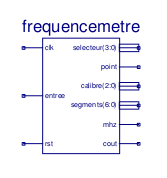
\includegraphics[scale=1]{freqa0.png}
	\caption{Component du projet fréquence}
\end{center}
\end{figure}

\subsection{Implémentation sur Nexys 2}
En chargent le .bit, l'utilisateur pourra utilisé le fréquencemètre.
\begin{figure}[H]
\begin{center}
	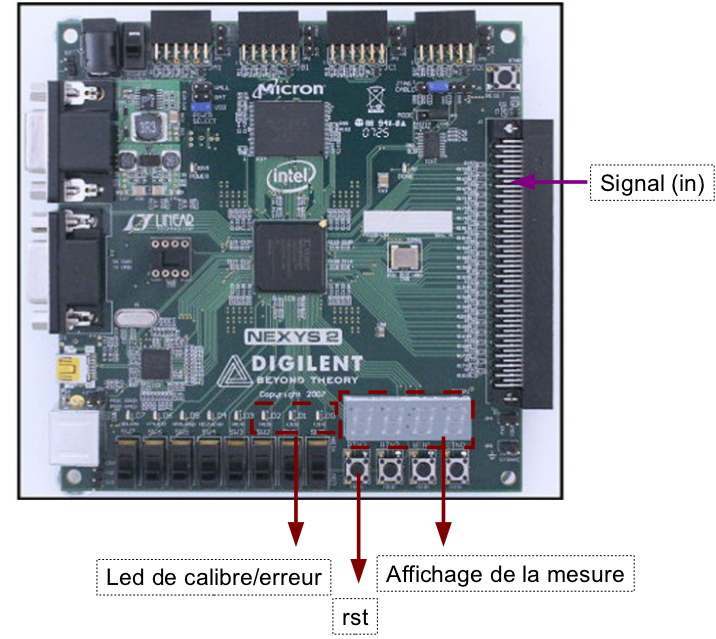
\includegraphics[scale=.5]{fpga.png}
	\caption{Implémentation sur carte Nexys 2}
\end{center}
\end{figure}

\subsection{Fichier contrainte}
L'utilisateur pourra édité le fichier de contraintes selon ses besoins et ressources disponible.
\lstinputlisting{../frequencemetre.ucf}
\newpage
\section{Extrait code vhdl}
\subsection{Module trouver-digit}
\lstinputlisting{../trouver_digit.vhd}
\end{document}
